\chapter{Module Loader}
\label{ch:ML}
\section{Linking and loading}
When the execution of a command M.P is requested, module M containing procedure P must be
loaded, unless it is already loaded because a command from the same module had been executed
earlier or if the module had been imported by another module before. Modules are available in the
form of so-called object files, generated by the compiler. The term loading refers to the transfer of the
module code from the file into main memory, from where the processor fetches individual instructions.
This transfer involves also a certain amount of transformation as required by the object file format on
the one hand and the storage layout on the other. A system typically consists of many modules, and
hence loading modules also involves linking them together, in particular linking them with already
loaded modules. Before loading, references to another module's objects are relative to the base
address of this module; the linking or binding process converts them into absolute addresses.
The linking process may require a significant amount of address computations. But they are simple
enough and, if the data are organized in an appropriate way, can be executed very swiftly.
Nevertheless, and surprisingly, in many OSes linking needs more time than compilation.
The remedy which system designers offer is a separation of linking from loading. A set of compiled
modules is first linked; the result is a linked object file with absolute addresses. The loader then
merely transfers the object file into main store.

We consider this an unfortunate solution. Instead of trying to cure an inadequacy with the aid of an
additional processing stage and an additional tool, it is wiser to cure the malady at its core, namely to
speed up the linking process itself. Indeed, there is no separate linker in the Oberon. The
linker and loader are integrated and fast enough to avoid any desire for pre-linking. Furthermore, the
extensibility of a system crucially depends on the possibility to link additional modules to the ones
already loaded by calls from any module. This is called dynamic loading. This is not possible with prelinked object files. Newly loaded modules simply refer to the loaded ones, whereas pre-linked files lead to the presence of multiple copies of the same module code.

Evidently, the essence of linking is the conversion of relative addresses as generated by the compiler
for all external references into absolute addresses as required during program execution. Before
proceeding, we must consider an additional complication. Assume that a module M1 is to be
compiled which is a client of (that is, it imports) module M0. The interface of M1 - in the form of a
symbol file - does not specify the entry addresses of its exported procedures, but merely specifies a
unique number (pno) for each one of them. The reason for this is that in this way the implementation
of M0 may be modified, causing a change of entry addresses, without affecting its interface
specification. And this is a crucial property of the scheme of separate compilation of modules:
changes of the implementation of M0 must not necessitate the recompilation of clients (M1). The
consequence is that the binding of entry addresses to procedure numbers must be performed by the
linker. In order to make this possible, the object file must contain a list (table) of its entry addresses,
one for each procedure number used as index to the table.

Similarly, the object file must contain a table of imported modules, containing their names. An
external reference in the program code then appears in the form of a pair consisting of a module
number (mno) - used as index to the import table (of modules) - and a procedure number (pno), used
as index to the entry table of this module.

Certain linkage information must not only be provided in each object file, but also be present along
with each loaded module's program code, because a module to be loaded must be linkable with
modules loaded at any earlier time without reading their object files again.

\section{Module representation}
The primary requirement is that a system must be represented in a form that allows to add new
modules quickly. What is a sensible representation for this purpose? The simplest solution that
comes to mind is a list of module blocks containing sections for the global data, for the program code,
and perhaps meta data for the linking process. The list is rooted in a variable global to the loader
module, here called Modules.
\begin{figure}
	\label{fig:4modules}
	\centering
	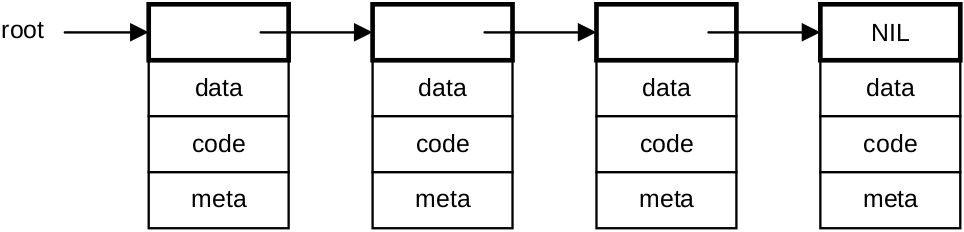
\includegraphics[width=\textwidth]{i/j}
	\caption{System of 4 modules}
\end{figure}

The first part, containing the link to the next module, is called the module descriptor. On the Oberon
System, it contains further links to the various sections of a module. The type Module is defined as
follows:
\begin{verbatim}
  TYPE Module = POINTER TO ModDesc;
    ModuleName = ARRAY 32 OF CHAR;
    ModDesc = RECORD
    name: ModuleName;
    next: Module;
    key, num, size, refcnt: INT;
    data,code,imp,cmd,ent,ptr: INT (*addresses*)
  END;
\end{verbatim}

key is the module's key used for version consistency checking. The key changes if, and only if, the
module's interface and thereby its symbol file changes. $num$ is the module's number, which is the
index of the module's entry in a global module table, referenced by the processor's MT register. The
invariant relationship is
\begin{verbatim}
  ModTable[mod.mno] = mod.data
\end{verbatim}

for all $mod$ in the module list. $size$ is the entire module block's size excluding the descriptor, and $refcnt$
is the number of other modules importing this module. This number is used to check whether a
module can be released by procedure $Modules.Free$.
\begin{figure}
	\label{fig:module-block}
	\centering
	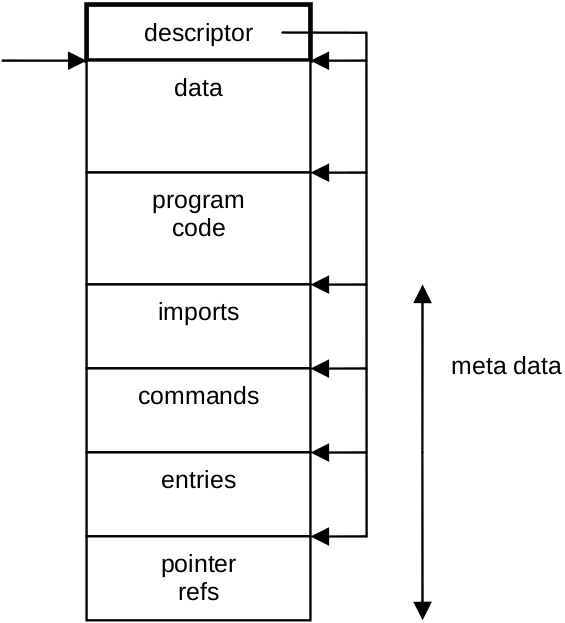
\includegraphics[width=.6\textwidth]{i/k}
	\caption{Module block headed by descriptor}
\end{figure}

The section with meta data follows the data and code areas and consists of several parts. Imports is
an array of the modules imported by this module, each entry being the address of the respective
module descriptor. Commands is a sequence of procedure identifiers followed by their offset in the
code section. This section is used when activating a command. Entries is an array of offsets of all
exported entities (including commands). This section is used by the loader itself for linking. Pointer
refs is an array of offsets of global pointer variables in the data section. These are used by the
garbage collector as the roots of graphs of heap objects in use.

\section{The linking loader}
The purpose of the loader is to read object files, and to transform the file representation of modules
into their internal image.

The loader is represented by procedure Load in module Modules. It accepts a name and returns a
pointer to the specified module's descriptor. It first scans the list searching for the named module.
Only if it is not present, the module is loaded and added to the list. Duplications therefore cannot occur.
\begin{verbatim}
  mod := root;
  WHILE (mod # NIL) & (name # mod.name) DO
    mod := mod.next
  END ;

  IF mod = NIL THEN (*load*)
    F := ThisFile(name);
    Files.Set(R, F, 0);
    ...
\end{verbatim}

First, the header of the respective object file is read. It specifies the required size of the block which is
allocated in the module area at the position indicated by the global variable AllocPtr. Then the list of
imports of the module being imported is read, and these module are imported. Evidently procedure
Load is used recursively. Because cyclic imports are excluded, recursion always terminates.
\begin{verbatim}
  Files.ReadString(R, impname); (*imports*)
  WHILE (impname[0] # 0X) & (res = 0) DO
    Files.ReadInt(R, impkey);
    Load(impname, impmod);
    import[nofimps] := impmod;
    importing := name1;
    IF res = 0 THEN
      IF impmod.key = impkey THEN
        INC(impmod.refcnt);
        INC(nofimps)
      ELSE
        error(3, name);
        imported := impname
      END
    END;
    Files.ReadString(R, impname)
  END
\end{verbatim}

The loading process stops, if a key mismatch is detected (err = 3). After successful loading of all
imports, the loading of the actual module proceeds by allocating a descriptor and then reading the
remaining sections of the file. The data is allocated (and cleared) and the code section is read in a
straight-forward way without alteration.

At the very end of the file three integers called fixorgP, fixorgD, and fixorgT are read. They are the
anchors of linked lists in the program code of instructions that need fixups. These fixups are
performed only after the entire file had been read. Traversing the P-list, the pairs mno-pno are
replaced by computed offsets in BL instructions (procedure calls). Traversing the D-list, addresses of
LDR instructions and instruction pairs are fixed up, and traversing the T-list, addresses of type
descriptors are computed and inserted. This low-level piece of code is shown below for call
instructions (BL). Those for the D-List and the T-list are analogous.
\begin{verbatim}
  adr := mod.code + fixorgP*4;
  WHILE adr # mod.code DO
    SYSTEM.GET(adr, inst);
    mno := inst DIV 100000H MOD 10H; (*decompose*)
    pno := inst DIV 1000H MOD 100H;
    disp := inst MOD 1000H;
    SYSTEM.GET(mod.imp + (mno-1)*4, impmod);
    SYSTEM.GET(impmod.ent + pno*4, dest);
    dest := dest + impmod.code;
    offset := (dest - adr - 4) DIV 4;    (*compose*)
    SYSTEM.PUT(adr,(offset MOD 1000000H)+0F7000000H);
    adr := adr - disp*4
  END;
\end{verbatim}

After the module has been loaded successfully, its initialization body is executed.
Apart from Load, module Modules also contains the procedures
\begin{verbatim}
PROC ThisCommand (mod: Module;
                      name: ARRAY OF CHAR): Command;
PROC Free (name: ARRAY OF CHAR);
\end{verbatim}

The former yields the procedure named name from module mod. It is used in $TextFrames.Call$ for
activating command procedures. The latter unloads the named module, i.e. removes it from the list of
loaded modules.

The frequent use of the low-level procedures $SYSTEM.GET$ and $SYSTEM.PUT$ is easily justified in
base modules such as the loader or device drivers. After all, here data are transferred into untyped
main storage.

\section{The toolbox of the loader}
User commands directed to the loader are contained in module $System$. The toolbox offers the following three commands:
\begin{verbatim}
  System.ShowModules
  System.ShowCommands modname
  System.Free {modname} ~
\end{verbatim}
The first command opens a viewer and provides a list of all loaded modules. The list indicates the
block length and the number of clients importing a module (the reference count). $ShowCommands$
opens a viewer and lists the commands provided by the specified module. The commands are
prefixed by the module name, and hence can immediately be activated by a mouse click. $Free$ is
called in order to remove modules either to regain storage space or to replace a module by a newly
compiled version. A module can be dispensed only if (1) it has no clients, and (2) if does not declare
any record types which are extensions of imported types.

\section{The Oberon object file format}
The name extension of object files is $.rsc$. Their syntax is the following:
\begin{verbatim}
  CodeFile = name key version size
  imports typedesc varsize strings code commands
          entries ptrrefs fixP fixD fixT body "O".
  imports = {modname key} 0X.
  typedesc = nof {byte}.
  strings = nof {char}.
  code = nof {word}.
  commands = {comname offset} 0X.
  entries = nof {word}.
  ptrrefs = {word} 0.
\end{verbatim}
$fixP$, $fixD$, $fixT$ are the origins of chains of instructions to be updated (fixed up). $body$ is the entry point
offset of the module $body$.